An Elliptic Billiard (EB) is a particle moving with constant velocity in the interior of an ellipse, undergoing elastic collisions against its boundary \cite{rozikov2018,sergei91}, Figure~\ref{fig:billiard-trajectories}. For any boundary location, a given exit angle (e.g., measured from the normal) may give rise to either a quasi-periodic (never closes) or $N$-periodic trajectory \cite{sergei91}, where $N$ is the number of bounces before the particle returns to its starting location. All trajectory segments are tangent to a confocal Caustic \cite{sergei91}. The EB is a special case of {\em Poncelet's Porism} \cite{dragovic11}: if one $N$-periodic trajectory can be found departing from some boundary point, any other such point will initiate an $N$-periodic, i.e., a 1d {\em family} of such orbits will exist. A classic result is that $N$-periodics conserve perimeter \cite{sergei91}.

\begin{figure}
    \centering
    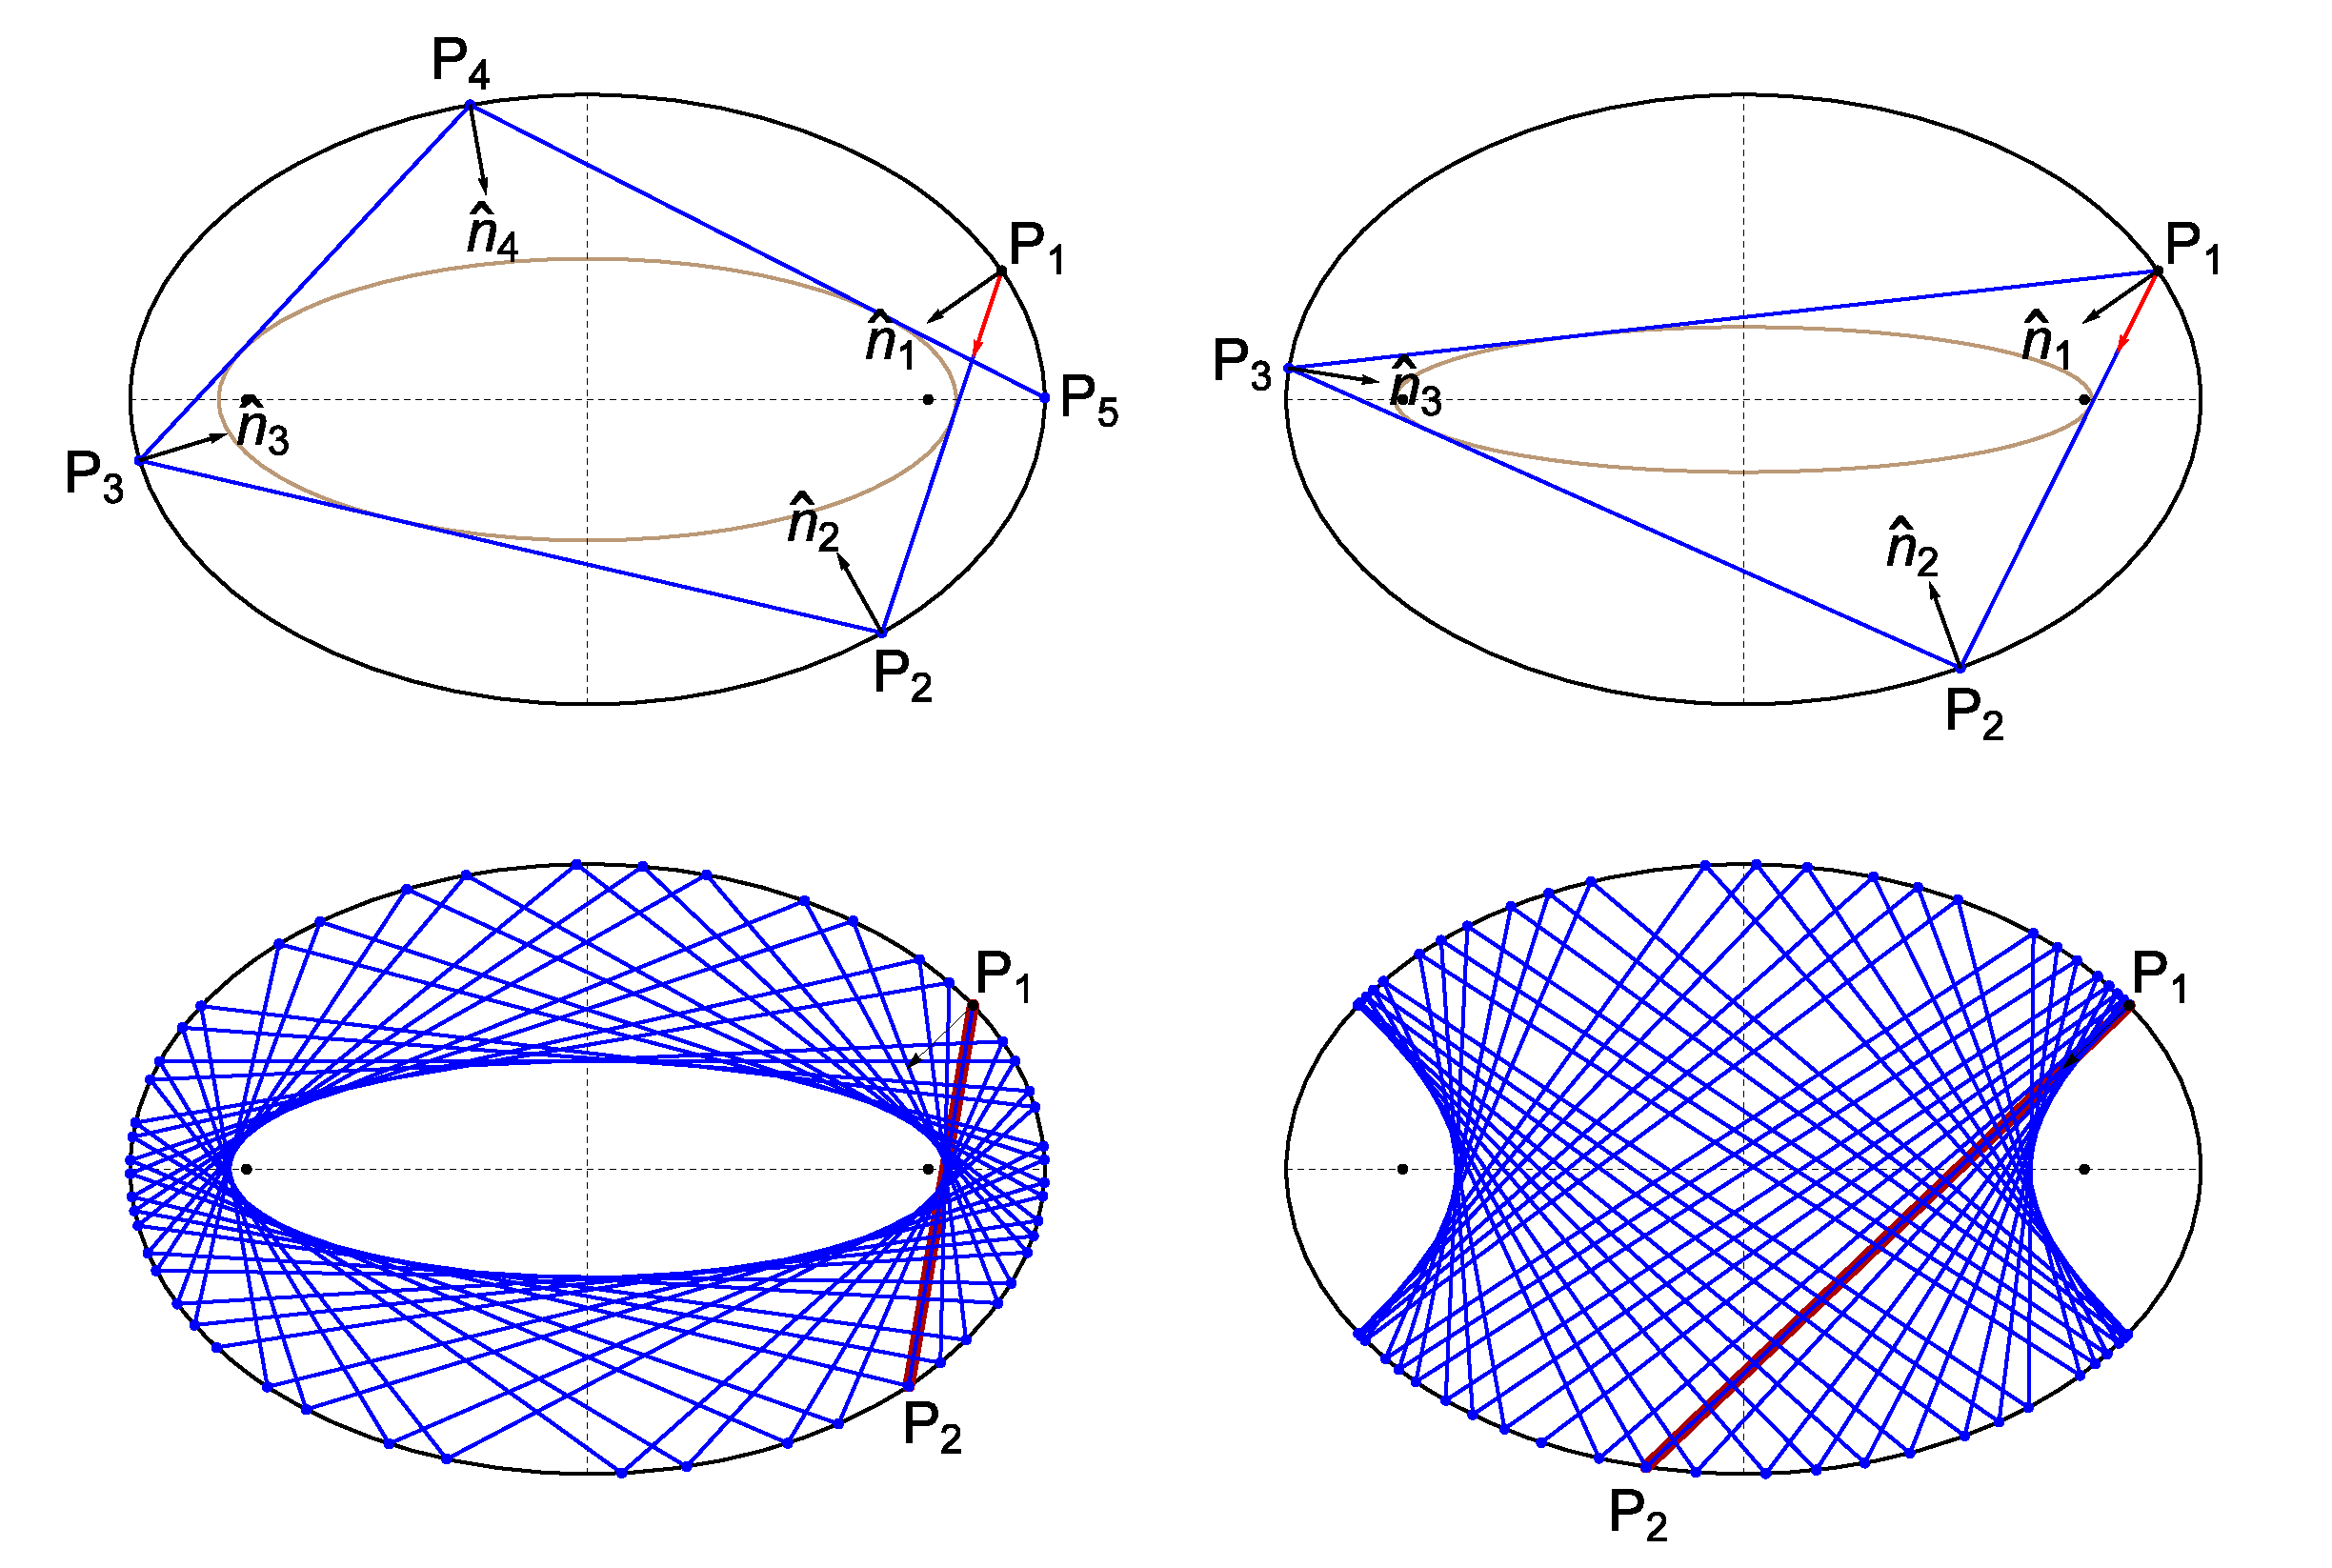
\includegraphics[width=\textwidth]{pics_1030_billiard_trajectories.eps}
    \caption{Trajectory regimes in an Elliptic Billiard, taken from \cite{reznik2020-intelligencer}. \textbf{Top left}: first four segments of a trajectory departing at $P_1$ and toward $P_2$, bouncing at $P_i, i=2,3,4$. At each bounce the normal $\hat{n}_i$ bisects incoming and outgoing segments. Joachimsthal's integral \cite{sergei91} means all segments are tangent to a confocal {\em Caustic} (brown). \textbf{Top right}: a 3-{\em periodic} trajectory. All 3-periodics in this Billiard will be tangent to a special confocal Caustic (brown). \textbf{Bottom}: first 50 segments of a non-periodic trajectory starting at $P_1$ and directed toward $P_2$. Segments are tangent to a confocal ellipse (left) or hyperbola (right). The former (resp. latter) occurs if $P_1P_2$ passes outside (resp. between) the EB's foci (black dots).}
    \label{fig:billiard-trajectories}
\end{figure}